\chapter{Partnering process}
\label{partnering}

The very first step after having the idea of introducing a new way for information to be retrieved in public places was to find a partner to realize it with. In order to find the most promising and suitable cooperation, appropriate properties would have to be defined and considered for each institution before partnering with any of them. Afterward, a suitable exhibit and an agreement on a design for the installation would be found.

%------------------------------------------------------------------------------
\section{Requirement analysis}
\label{partnering_requirement}

To determine an ideal partner for a cooperation, a mutual beneficial system of needs and demands had to be established. Therefore, each party's needs and offerings were identified. As Table \ref{tab:museums_needs_demand} shows, three major criteria were determined. Possible cooperations would be based on those criteria. In addition, special characteristics would be considered as well.

\begin{table}[h]
	\centering
	\begin{tabular}{ bl !{\vrule width 1pt} nl nl}
		\rowstyle{\bfseries}
												& Museum 										& Me \\
		\toprule
		\textbf{Needs} 			& Improvement / Innovation	& Access to a public space \\
												&														&	with exhibits and visitors \\		
												& New group of visitors			& Authentic content \\
												& Publicity	/ Awareness			& Potential test subjects \\
		\hline
		\textbf{Offerings}	& A public space						& Technological expertise \\ 
												& Factual expertise		 			& Development and testing \\ 
												& Resources									& Motivation \\ 
	\end{tabular}
	\caption{Needs and Demand.}
	\label{tab:museums_needs_demand}
\end{table}

Museums want to get people interested in their respective topics. Thus, reaching more people and raising awareness is one of their main interests. A good way to attract new groups of visitors is to offer something unique and innovative. Although there are companies offering services like guide- or information-systems, they are either cosmetic, expensive or high-maintenance. On the other hand, a museum has valuable offerings. Usually, they have a budget for renovation and improvements. The staff is highly skilled and experienced concerning the exhibits and visitors' behavior around them. Finally, a museum offers a public space, where a system can be tested under natural conditions.
\\ 
The Bauhaus-Universität and specifically the chair for \ac{HCI} as well as myself wanted the final system to work in a real-life environment, but not as a lab-study alone. Hence, we needed access to a public place in order to reach a broad variety of people. Those would be unbiased toward the nature of interaction and content as well. Meanwhile, we could provide our knowledge of interaction design and the suitability of contemplable technologies. And lastly, I was highly motivated to develop a working system.
\\
After finding a cooperation partner, a \ac{FSD} would be made, which includes the system's properties ordered by necessity. In addition, a contract between all parties would be drawn up to register each party's contributions and obligations.

%\paragraph{Annotations}
%
%\begin{itemize}
	%\item 'What do we have to offer?'
	%\begin{itemize}
		%\item Expertise
		%\item Time
		%\item Motivation
	%\end{itemize}
	%\item 'What do we need?'
	%\begin{itemize}
		%\item A museum
		%\item Access
		%\item Public (for evaluation)
	%\end{itemize}
	%\item 'What should the museum be offering?'
	%\begin{itemize}
		%\item Location ('A museum')
		%\item Staff's expertise
		%\item Hardware
		%\item Access (for evaluation)
	%\end{itemize}
	%\item 'What does the museum want?' \textit{better: need}
	%\begin{itemize}
		%\item A working Improvement of their exhibition
	%\end{itemize}
	%\item Pflichtenheft
	%\item Contract
	%\item Further Cooperation
%\end{itemize}

%-----------------------------------------------------------------------------

\section{Potential partner museums}
\label{partnering_investigation}

According to \ac{MVT}~\cite{ThueringerMuseumsverbandOrte} there are more than 50  museums in Weimar within a few kilometers distance from the town. Table \ref{tab:museums_amounts} only shows museums registered at the \ac{MVT} and the three towns with the most of them. Other towns have between one and six registered museums. Further, it is most likely that there are more museums than those in this list. It provides a good starting point, though.

\begin{table}[h]
	\centering
	\begin{tabular}{ bl !{\vrule width 1pt} nr }
		\rowstyle{\bfseries}
		Town		& Museums \\
		\toprule
		Weimar	& 26 \\ 
		Erfurt 	& 12 \\ 
		Jena 		& 12 \\ 
	\end{tabular}
	\caption{Museums in and around Weimar.}
	\label{tab:museums_amounts}
\end{table}

Regarding the high amount of museums in Weimar alone, it seemed promising to start looking for a suitable cooperation partner right here. Since 26 museums are too many to investigate thoroughly, a preselection had to be made. In the first step, the focus was on flexibility. This meant, only a small administrative apparatus could guarantee fast decisions and less organizational meetings with boards and other decision makers. Hence, all the \textit{Klassikstiftung}'s museums were crossed of the list, narrowing it down to only 10 remaining candidates. Next, and after some further research, museums with less interesting topics or inconvenient concepts were withdrawn. This included the tiny \textit{umbrella museum} and \textit{Weimar Haus}, a place glutted with animatronics. Afterward, the list of candidates was down to five (see Table \ref{tab:museums_finalists}). A personal visit to each of these museums was indispensable now.

\begin{table}[h]
	\centering
	\begin{tabular}{ bl }
		\rowstyle{\bfseries}
		Museum \\
		\toprule
		Deutsches Bienenmuseum \\
		Kirms-Krakow-Haus \\
		Museum für Ur- und Frühgeschichte Thüringens \\ 
		Palais Schardt \\
		Pavillon Presse \\
	\end{tabular}
	\caption{Remaining cooperation candidates.}
	\label{tab:museums_finalists}
\end{table}

Gathering impressions in person was a process of three stages. In the first stage, I would visit a museum and noted its technical and pedagogical equipment. This was directly followed by the next stage, an informal introduction to some of the staff  containing a chat about my plans and the respective person's attitude towards them. The final stage was a formal introduction-meeting between my professor, me and the administrative staff of each museum, that had expressed serious interest. This serious interest wasn't shown by the Kirms-Krakow-Haus and the Pavillon Presse. Hence, the aforementioned meeting only took place at the Deutsche Bienenmuseum, Museum für Ur- und Frühgeschichte Thüringens and Palais Schardt. We introduced ourselves at each venue, because a discussion about what might be done was more efficient directly on site.  

%\paragraph{Annotations}
%
%\begin{itemize}
	%\item Project process: Partnering
	%\\
	%\item Preselection of possible partners
	%\item Criteria
	%\begin{itemize}
		%\item Proximity
		%\begin{itemize}
			%\item Thüringer Museumsverband~\cite{ThueringerMuseumsverbandOrte} (Weimar, Jena, Erfurt, Apolda have 50 museums)
			%\item Weimar alone has 26, and probably more than that
		%\end{itemize}
		%\item Flexibility
		%\begin{itemize}
			%\item Little administrative apparatus $\to$ no Klassikstiftung
			%\item Making (faster) decisions, due to less administration (Gremien)
			%\item Direct connection to chairs
			%\item Willingness for cooperation
		%\end{itemize}
		%\item Open-mindedness
		%\begin{itemize}
			%\item Many different and realizable topics
			%\item Excitable for and capable of new Ideas
			%\item Willingness for change
		%\end{itemize}
		%\item Attractiveness
		%\begin{itemize}
			%\item Topic(s)
			%\item Realizability of the interaction-idea(s)
			%\item Guts
		%\end{itemize}
	%\end{itemize}
	%\item 'Supply and demand'
	%\begin{itemize}
		%\item Necessities to realize the idea
		%\item Who provides what $\to$
	%\end{itemize}
%\end{itemize}

%-----------------------------------------------------------------------------

%\paragraph{Annotations}
%
%\begin{itemize}
	%\item Visit preselected museums
	%\begin{itemize}
		%\item Taking notes
		%\item Taking photos
	%\end{itemize}
	%\item Getting an Overview $\to$ (Im)Possibilities
	%\begin{itemize}
		%\item Some Criteria for realizability
		%\begin{itemize}
			%\item Atmosphere (outdated vs. innovative tendencies)
			%\item Space for an installation
			%\item Number of other visitors
		%\end{itemize}
	%\end{itemize}
	%\item Establish a first contact
	%\begin{itemize}
		%\item Talk to staff
		%\item Make an appointment with executives (board)
	%\end{itemize}
%\end{itemize}

%-----------------------------------------------------------------------------

\section{Decision for a partner museum}
\label{partnering_decision}

A formal introduction-meeting went as follows: First, I explained some of my previous projects, related installations in other museums and the general intent of the professor's chair. Next, the staff explained their museum's concept and which subject area they would like to emphasize. After that, we discussed potential concepts. Those ranged from augmentations of existing exhibits to completely new installations.

\paragraph{Deutsches Bienenmuseum} 

The museum is run by the beekeepers association of Thuringia. The staff we encountered was very skilled with the craft of beekeeping, but less professional concerning museum education and design. A part of the exhibition of the museum is shown in Figure \ref{fig:bienenmuseum}. They listened to my remarks and we had an inspiring discussion about potential topics and their feasibility. Unfortunately, the association's chairman and we could not agree on a specific project. Also, because bees hibernate, visitor attendances are seasonal and also fluctuant. Hence, the Deuschte Bienenmuseum was out of the picture.
\begin{figure}[H]%
\includegraphics[width=\columnwidth]{../pics/bienenmuseum.eps}%
\caption{Impressions of the Deutsche Bienenmuseum.}%
\label{fig:bienenmuseum} 
\end{figure}

\paragraph{Palais Schardt} 

The venue is owned by a family, which exhibits multiple collections of art and crafts as well as the building itself. In addition, they operate a cafe and use the adjacent hall for events. The husband is a restorer by trade and gives talks about the building and its historic significance, while his wife handles planning and the cafe. The Goethepavillon shown in Figure \ref{fig:schardt_pavilon} is the highlight of the venue. 
\begin{figure}[H]%
\includegraphics[width=\columnwidth]{../pics/palais_schardt.eps}%
\caption{Impressions of the Goethepavillon at Palais Schardt.}%
\label{fig:schardt_pavilon} %
\end{figure}
Further, events at the ball room are regular, and the cafe supplies the venue with casual customers and visitors. Both owners were very interested in a cooperation and had some ideas for installations. But monument protection of the building and minor financial issues complicated the feasibility. Therefore, Palais Schardt also had to go. 

\paragraph{Museum für Ur- und Frühgeschichte Thüringens} 

Since the state office for preservation of historical monuments and archeology of Thuringia is the bearer of the museum, all personnel is very competent at their field of work. In addition, the museum employs special staff, that maintains the exhibition, gives tours and is present for arising topical questions during opening hours. Classes of 5th and 6th grade visit regularly for field trips as well as visitors from all age groups. The exhibition was already altered by several media installations. Moreover, the director was very enthusiastic from the first meeting on and had several ideas, of which exhibits to emphasize.
\begin{figure}[H]%
\includegraphics[width=\columnwidth]{../pics/muft.eps}%
\caption{Impressions of the Museum für Ur- und Frühgeschichte Thüringens.}%
\label{fig:muft} %
\end{figure}
Summarizing, the Deutsche Bienenmuseum and Palais Schardt were deemed less interesting and lacking feasibility. The Museum für Ur- und Frühgeschichte Thüringens was chosen as the cooperation partner, because it checked the most boxes of the previous Requirement Analysis (see Chapter \ref{partnering_requirement}), while the others lacked at least once in the \textit{Needs}- or \textit{Offerings}-category. It was the most professional and ambitious candidate with promising resources and conditions.

%\paragraph{Annotations}
%
%\begin{itemize}
	%\item Offical introduction at the museum
	%\begin{itemize}
		%\item Personal
		%\begin{itemize}
			%\item Projects
			%\begin{itemize}
				%\item Perceiving AR (Psychophysiologie und Wahrnehmung - Huckauf)
				%\item pEYEwrite (Psychophysiologie und Wahrnehmung - Huckauf)
				%\item Schlender (Usability - Bertel)
				%\item Neural Control (Vernetzte Systeme - Schatter)
				%\item KickFlickable Interfaces (HCI - Hornecker)
			%\end{itemize}
			%\item Bachelor Thesis (VR - Fröhlich)
			%\item Skills
			%\begin{itemize}
				%\item Interdisciplinary work experience (Schlender, KickFlickable Interfaces)
				%\item Multiple programming Languages and their (dis-)advantages for a project (Schlender) $\to$ Chapter \ref{conception} Conception
				%\item Interface Design 
				%\item User Experience
				%\item Rapid Prototyping
			%\end{itemize}
		%\end{itemize}
		%\item Present requirements see \ref{museums_requirement}
	%\end{itemize}
	%\item Brainstorming
	%\begin{itemize}
		%\item Museum-staff: 'Emphases'
		%\item Me: 'Possible solutions'
	%\end{itemize}
%\end{itemize}

%-----------------------------------------------------------------------------

%\subsection*{Old version}
%
%In order to finding a museum to cooperate with several steps had to be made. They included getting an overview of all museums in Weimar, finding several candidates for that cooperation, scouting those candidates and getting in contact with the most promising of them, and, finally, discussing possible concepts within their exhibitions.
%\\
%The first step was to find out about all the museums in Weimar and close by. So I looked them up on the website of Museumsverband Thüringen~\cite{ThueringerMuseumsverbandOrte} see Table \ref{tab:museums_amounts}, where there is a list of all members with links to further information. This list included museums in Weimar, Jena and Erfurt. Some were run privately, others by a foundation or a club, and a few by a public owner. Since there was a total of fifty museums and half of them in Weimar alone, there had to be a preselection.
%
%\begin{table}[]
	%\centering
	%\begin{tabular}{ bp{5em} nr }
		%\rowstyle{\bfseries}
		%Location & Amount \\
		%\toprule
		%Weimar & 26 \\ 
		%Erfurt & 12 \\ 
		%Jena & 12 \\ 
		%Apolda & 1 \\ 
		%\bottomrule
		%Total & 51 \\ 
	%\end{tabular}
	%\caption{Museums in and around Weimar.}
	%\label{tab:museums_amounts}
%\end{table}
%
%Hence, as the following step, only museums in Weimar were chosen. In addition, the museums run by Klassikstiftung were taken out of consideration, for the foundation seemingly being too big and too inflexible concerning innovation in their historic premises. Some very small museums were struck off the list as well. This left four candidates remaining. They were Pavillon Presse, Pallais Schardt, Bienenmuseum and Museum für Ur- und Frühgeschichte Thüringens.
%\\
%The next step was to get some first hand experience of each of the aforementioned museums. So, I went to visit all of them. During the visit I took notes and pictures of the exhibitions. Afterward, I talked to some staff members, explained what I was about to do, and arranged an appointment for an official introduction later on.
%\\
%The first visit was to the Bienenmuseum. It is run by a club of beekeepers and displays exhibits of beekeeping throughout the ages and several cultures. The exhibition is mainly conventional with vitrines and open exhibits. Moreover, they offer workshops, in which attendees learn more about bees in general, 'making' honey and even dipping our pouring candles.
%\\
%Pallais Schardt was the second visit. It is the historical home of the Schardt family, a very influential family at the court of Sachsen-Weimar. This place is owned by the Brinkmann family and run aside a cafe with traditional pastries from that particular era. Mr. Brinkmann is giving tours around the premisses and explains the building's significance in close contact to historical events. In addition, the saloon and other rooms can be rented for festivities.
%\\
%Right next to Pallais Schardt is Pavillon Presse. It used to be a printery and now accomodates printing presses and equipment from all ages. The museum is privately run by a foundation and volunteers. This museum was struck of the list immediately after the visit, for being to capricious to work with.
%\\
%The final visit was to the Museum für Ur- und Frühgeschichte Thüringens. There, artifacts from fossils, which a millions of years old, to medieval times are exihibited. The museum was overhauled in 1999 and thus, has a modern touch already. It is owned and run by the Thüringisches Landesamt für Denkmalpflege und Archäologie.
%
%\begin{figure}[H] % [H] -> Here!
	%\centering
	%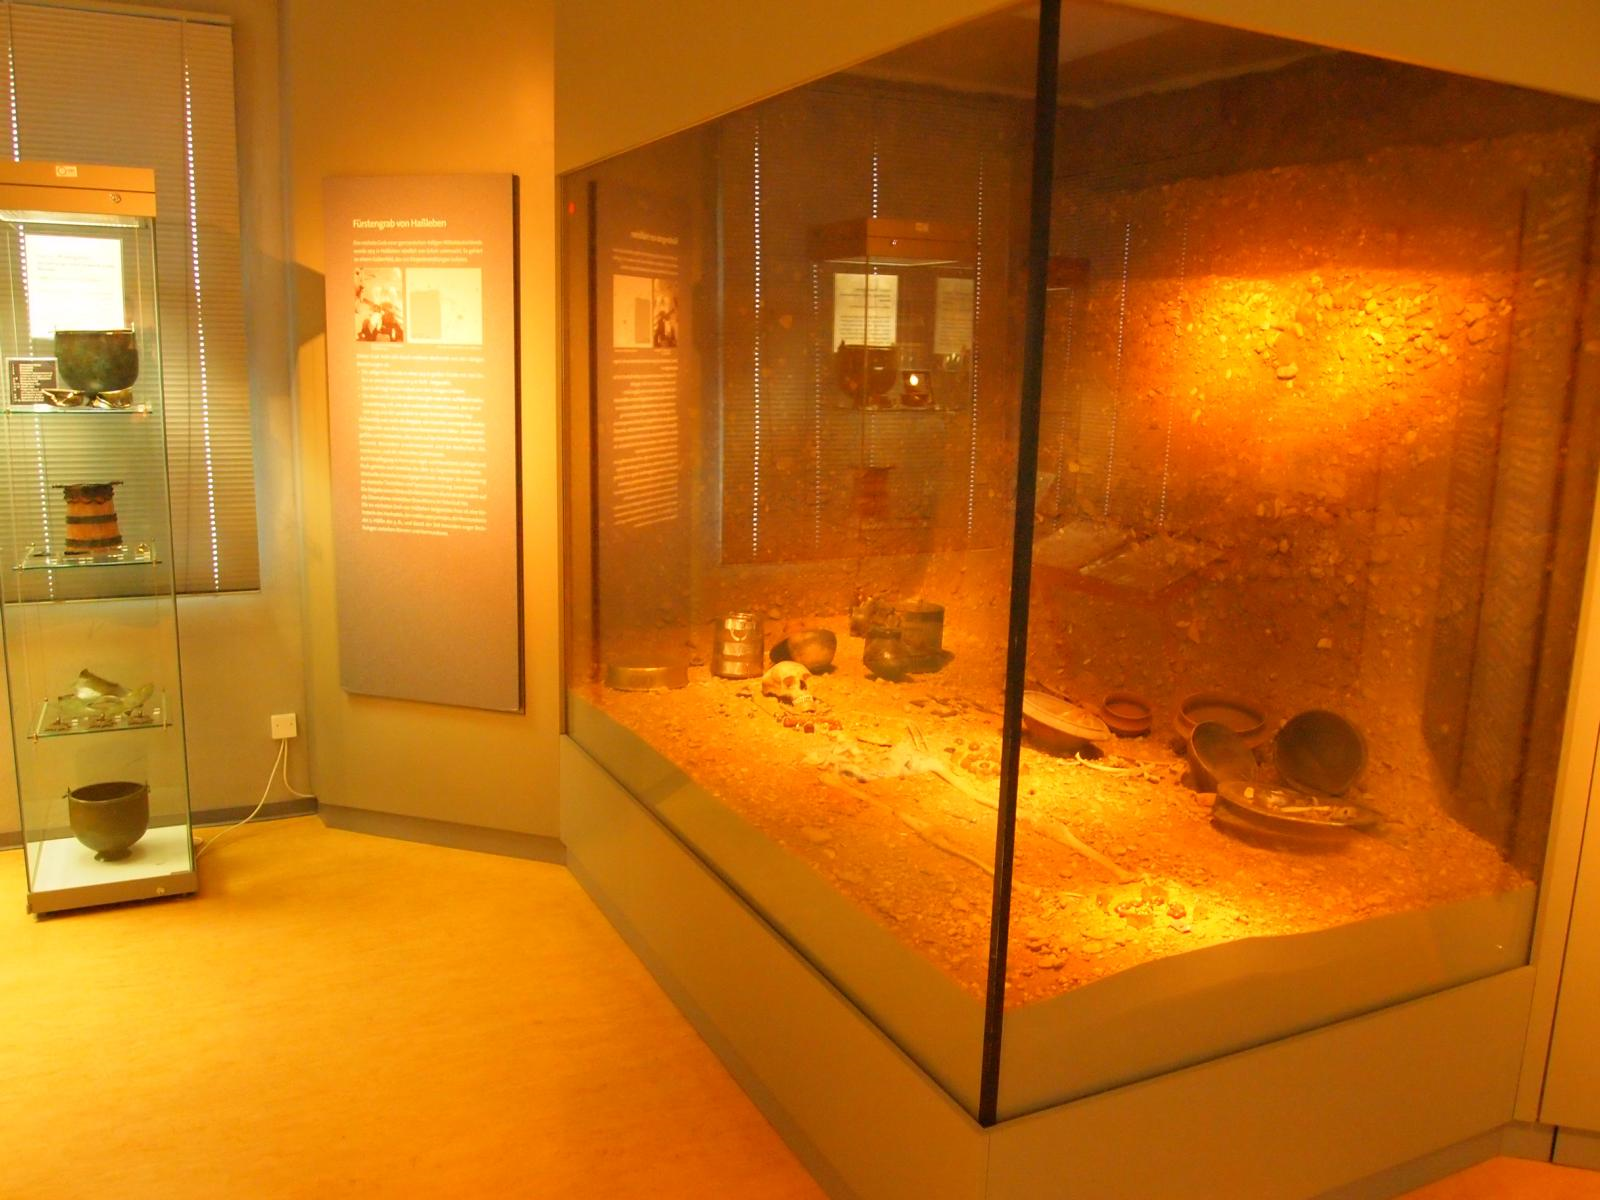
\includegraphics[width=1.0\textwidth]{../pics/Original.png}
	%\caption{Original display of the Haßleben grave.}
	%\label{fig:museums_original}
%\end{figure}
%
%After those field trips, I fashioned a presentation, in which I would introduce myself and previous projects I participated in. Later on in the meeting, I would show pictures of the museums in Limmerick and Vienna and explained the work, which had been done there. Finally, I prepared a short presentation of the Microsoft Gadgeteer-system and some of its capabilities. Following my presentation, the attending museum-staff, my professor end I discussed possible deployment scenarios. During the brainstorming the museum-officials named exhibits, which could or rather should receive more attention, whilst me and my professor suggested fitting solutions or explained further technological possibilities.
%\\
%At Pallais Schardt, the owners were very interested in technology, but they could not imagine how and where to make use of it. The best thing we could come up with was a guided tour. Thus, I was invited to one of their soirees with classical music and a tour of the house, in order to making up my own mind. Although it was very interesting, nothing ground-breaking arose.
%\\
%At Museum für Ur- und Frühgeschichte, the director was very fascinated by the demo and immediately came up with several exhibits, which seemed fitting to him. Yet, his optimism had to be reined a little. Some of the tasks he had in mind were unfortunately not realizable with the tools I had in hand.
%\\
%At Bienenmuseum, there were two main topics. First, social interaction of bees. For instance, bees dance to communicate the direction of plenty resources. Second, bees' perception of their environment. Bees see in another spectrum than we do and they can smell a lot better than us. In the end of our meeting, we were discussing about a virtual bee hive. This installation would be able
%to simulate the behavior of a bee colony according to some certain inputs, which could be made by visitors.
%\\
%The final decisions were made after working out several key criteria for the best possible cooperation. Those were common criteria every museum could or could not meet and special criteria, which could also tip the scales. Three common criteria were identified. First of all, the amount and age of visitors was very important. Since the prototype had to be evaluated, a sufficient number of potential test subjects with a certain grade of affinity for technology would be needed. Second and not much less important, was the size and quality of the staff. If there was no expert of the museum's subject, who was able to work together with me, the project would be a fail. The third criteria was plainly budget. At some point, additional electronics and/or other equipment would be necessary. The special criteria more or less had an influence on the aforementioned main criteria. For example, monument protection, seasons, and motivation were some of them. First, Bienenmuseum had to go, because the club's chairman was not very fond of our discussions. Furthermore, the staff was not particularly professional and seemed to run the museum more as a hobby. The fact, that the museum has a large variety of visitors was a big plus, which was neutralized with the other fact, that bees are seasonal, and so are the according numbers of visitors. This makes an evaluation rather difficult, for not providing a constant number of test subjects.
%\\
%Finally, Pallais Schardt was struck from the list. Although, its owner was a restorer by trade, very approachable, and there were lots of events at the cafe, it had some corresponding cons as well. The building ant its historic role was very interesting, yet is a landmark. Thus, it must not be altered in any form, which might prove hard later on. The many people visiting the cafe are mostly 50 years an older. Hence, their abilities to understand and use technology as intended could be too much a risk during evaluation. Sadly, it is just a cafe and not a museum.
%\\
%The last item on the list is the Museum für Ur- und Frühgeschichte Thüringens. The major con was the planned exhibition, which leaves not much space for alterations. But, it is controlled by regional authorities. Hence, there is a budget for innovation projects. Moreover, the staff at the museum is interested in innovation and highly qualified in their field of expertise.
